\documentclass[aspectratio=169,11pt]{beamer}
\def\courseweek{6}
% Shared style for the Introduction to Information Geometry lecture slides.
% Compile the lecture .tex files from this directory.
\providecommand{\courseweek}{1}
\usepackage[T1]{fontenc}
\usepackage[utf8]{inputenc}
\usepackage[sc]{mathpazo}
\renewcommand{\sfdefault}{lmss}
\renewcommand{\ttdefault}{lmtt}
\usepackage{amsmath,amssymb,mathtools}
\usepackage{tikz}
\usetikzlibrary{arrows.meta,calc,positioning}
\usepackage{pgfplots}
\pgfplotsset{compat=1.18}
\usepackage{booktabs}

\definecolor{courseink}{HTML}{173749}
\definecolor{coursemuted}{HTML}{526674}
\definecolor{courseteal}{HTML}{0E7287}
\definecolor{coursecopper}{HTML}{B66B43}
\definecolor{courseline}{HTML}{D4E0E3}
\definecolor{coursepale}{HTML}{EFF5F5}

\setbeamercolor{normal text}{fg=courseink,bg=white}
\setbeamercolor{structure}{fg=courseteal}
\setbeamercolor{frametitle}{fg=courseink,bg=white}
\setbeamercolor{title}{fg=courseink}
\setbeamercolor{subtitle}{fg=coursemuted}
\setbeamercolor{block title}{fg=courseink,bg=white}
\setbeamercolor{block body}{fg=courseink,bg=white}
\setbeamercolor{alerted text}{fg=coursecopper}
\setbeamerfont{title}{family=\rmfamily,series=\bfseries,size=\fontsize{32}{37}}
\setbeamerfont{frametitle}{family=\rmfamily,series=\bfseries,size=\fontsize{26}{31}}
\setbeamerfont{normal text}{size=\fontsize{18}{22}}
\setbeamerfont{subtitle}{size=\fontsize{17}{21}}
\setbeamersize{text margin left=0.78cm,text margin right=0.78cm}
\setbeamertemplate{navigation symbols}{}
\setbeamertemplate{itemize items}[circle]
\setbeamertemplate{enumerate items}[default]
\setbeamertemplate{blocks}[default]
\setlength{\parskip}{0.22em}
\setbeamertemplate{footline}{%
  \leavevmode\hbox to \paperwidth{\hspace{.78cm}%
  {\color{coursemuted}\fontsize{8.5}{10}\selectfont Introduction to Information Geometry \hspace{.32cm} / \hspace{.32cm} Week \courseweek}%
  \hfill{\color{coursemuted}\fontsize{8.5}{10}\selectfont \insertframenumber\hspace{.17cm}/\hspace{.17cm}\inserttotalframenumber}\hspace{.78cm}}%
  \vskip.17cm
}
\setbeamertemplate{frametitle}{%
  \vspace{.13cm}
  \insertframetitle\par
  \vspace{.08cm}
}
\setbeamertemplate{title page}{%
  \vspace*{1.00cm}
  {\color{courseteal}\fontsize{10}{13}\selectfont\bfseries
  INTRODUCTION TO INFORMATION GEOMETRY\par}
  \vspace{.40cm}
  {\usebeamerfont{title}\usebeamercolor[fg]{title}\inserttitle\par}
  \vspace{.22cm}
  {\usebeamerfont{subtitle}\usebeamercolor[fg]{subtitle}\insertsubtitle\par}
  \vfill
  {\color{coursemuted}\fontsize{13}{16}\selectfont Christopher Lee\par}
  \vspace{.34cm}
}

\pgfplotsset{
  courseplot/.style={
    width=11.05cm,
    height=5.15cm,
    axis line style={coursemuted!75},
    tick style={coursemuted!65},
    ticklabel style={font=\scriptsize,color=coursemuted},
    label style={font=\normalsize,color=courseink},
    grid=major,
    major grid style={courseline!70,line width=.4pt},
    line width=1.45pt,
    legend style={font=\small,draw=none,fill=none,at={(.98,.03)},anchor=south east},
    clip=true
  }
}

\newcommand{\highlightmath}[1]{{\color{courseteal}#1}}
\newcommand{\thinrule}{\par\vspace{.25cm}{\color{courseline}\rule{\linewidth}{.8pt}}\par}

% A one-dimensional state space.  x=0 and x=1 are placed at 0 and 9 units.
\newcommand{\stateinterval}[1]{%
 \begin{tikzpicture}[x=1cm,y=1cm]
   \draw[courseink,line width=1.25pt] (0,0)--(9,0);
   \foreach \pos/\lab in {0/0,9/1} {
     \fill[courseink] (\pos,0) circle(2.7pt);
     \node[below=9pt,text=coursemuted] at (\pos,0) {\(\lab\)};
   }
   #1
 \end{tikzpicture}%
}

% Paired pages are separate frames in the PDF, with matching titles.
% Supply the whole frame body for each version; the instructor may edit them
% independently without changing overlay logic.
\newcommand{\coursepair}[3]{%
  \begin{frame}{#1}#2\end{frame}%
  \begin{frame}{#1}#3\end{frame}%
}

% Equilateral representation of the categorical simplex, in barycentric
% coordinates with vertices A=(0,0), B=(1,0), C=(1/2,sqrt(3)/2).
\newcommand{\coursesimplex}[1]{%
 \begin{tikzpicture}[scale=4.9]
  \fill[coursepale] (0,0)--(1,0)--(.5,.8660254)--cycle;
  \draw[courseink,line width=.65pt] (0,0)--(1,0)--(.5,.8660254)--cycle;
  \node[below left,font=\small] at (0,0) {A};
  \node[below right,font=\small] at (1,0) {B};
  \node[above,font=\small] at (.5,.8660254) {C};
  #1
 \end{tikzpicture}%
}

\title{Relative Entropy and Prediction}
\subtitle{Week 6 \(\cdot\) Lecture 1}
\date{}
\begin{document}
\begin{frame}[plain]\titlepage\end{frame}

\begin{frame}{Predicting observations with a model}
Suppose observations follow the law \(Q=(q_i)\), while our
predictive model is \(P=(p_i)\).
\vspace{.4cm}
Under logarithmic loss, outcome \(i\) costs \(-\ln p_i\).
\vspace{.37cm}
Its expected loss is the cross-entropy
\[
\highlightmath{\operatorname{CE}(Q,P)=-\sum_i q_i\ln p_i}.
\]
\end{frame}

\begin{frame}{Relative entropy is excess log loss}
Using the generating law itself gives expected loss \(H(Q)\).
The additional loss from using \(P\) is
\vspace{.46cm}
\[
\highlightmath{D(Q\|P)=\operatorname{CE}(Q,P)-H(Q)}
\]
\vspace{.25cm}
\[
=\highlightmath{\sum_i q_i\ln\frac{q_i}{p_i}}.
\]
\vspace{.43cm}
The first argument supplies the averaging probabilities.
\end{frame}

\coursepair{The cost of an equal-probability prediction}{
Take the generating law \(Q=(\frac34,\frac14)\)
and model \(P=(\frac12,\frac12)\).
\vspace{.38cm}
Compute
\[
D(Q\|P)=\frac34\ln\frac{3/4}{1/2}
+\frac14\ln\frac{1/4}{1/2}.
\]
}{
Take the generating law \(Q=(\frac34,\frac14)\)
and model \(P=(\frac12,\frac12)\).
\vspace{.38cm}
The relative entropy is
\[
\highlightmath{D(Q\|P)=\frac34\ln\frac32
+\frac14\ln\frac12\approx0.1308}.
\]
\vspace{.2cm}
This is the excess expected loss in nats per observation.
}

\begin{frame}{The direction of the comparison matters}
Reversing the two arguments changes the averaging law.
\vspace{.36cm}
For \(P=(\frac12,\frac12)\), \(Q=(\frac34,\frac14)\),
\[
D(P\|Q)=\frac12\ln\frac23+\frac12\ln2
=\highlightmath{\frac12\ln\frac43}.
\]
\vspace{.36cm}
\[
D(P\|Q)\approx0.1438\ne D(Q\|P)\approx0.1308.
\]
\vspace{.24cm}
KL divergence is a directed comparison.
\end{frame}

\begin{frame}{Why divergence is nonnegative}
The inequality \(\ln u\leq u-1\) holds for every \(u>0\).
\vspace{.42cm}
Apply it to \(u=p_i/q_i\), multiply by \(q_i\), and sum:
\[
\begin{aligned}
D(Q\|P)&\geq\sum_iq_i\left(1-\frac{p_i}{q_i}\right)\\
&=\sum_i(q_i-p_i)=0.
\end{aligned}
\]
\vspace{.37cm}
Equality holds precisely when \(P=Q\).
\end{frame}

\begin{frame}{Divergence on the Bernoulli interval}
Fix \(Q=(.75,.25)\); vary \(P=(p,1-p)\).
\vspace{-.18cm}
\begin{center}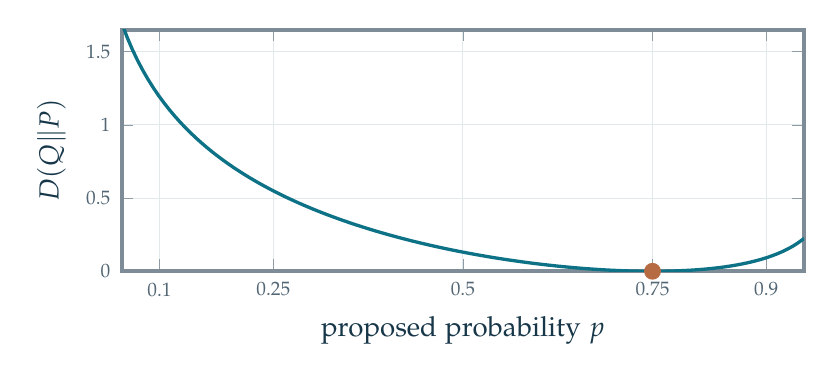
\begin{tikzpicture}
\begin{axis}[courseplot,width=10.25cm,height=4.65cm,
 xmin=.05,xmax=.95,ymin=0,ymax=1.65,
 xlabel={proposed probability $p$},ylabel={$D(Q\|P)$},
 xtick={.1,.25,.5,.75,.9},ytick={0,.5,1,1.5}]
\addplot[courseteal,very thick,domain=.05:.95,samples=130]
{.75*ln(.75/x)+.25*ln(.25/(1-x))};
\addplot[only marks,coursecopper,mark=*,mark size=2.3pt]coordinates{(.75,0)};
\end{axis}\end{tikzpicture}\end{center}
\end{frame}

\begin{frame}{Support determines finiteness}
If the generating law assigns positive probability to an outcome
that the predictive law assigns probability zero, then
\[
\highlightmath{D(Q\|P)=+\infty}.
\]
\vspace{.50cm}
Finite divergence requires
\[
\operatorname{supp}(Q)\subseteq\operatorname{supp}(P).
\]
\end{frame}

\coursepair{A boundary comparison}{
Let \(Q=(1,0)\) and \(P=(\frac12,\frac12)\).
\vspace{.50cm}
Calculate \(D(Q\|P)\) and determine \(D(P\|Q)\).
\vspace{.34cm}
\[
D(Q\|P)=\;?,\qquad D(P\|Q)=\;?.
\]
}{
Let \(Q=(1,0)\) and \(P=(\frac12,\frac12)\).
\vspace{.50cm}
The directed comparisons are
\[
\highlightmath{D(Q\|P)=\ln2},\qquad
\highlightmath{D(P\|Q)=+\infty}.
\]
\vspace{.34cm}
The second model rules out a possible generated outcome.
}

\begin{frame}{Observed frequencies become a model}
If a sample contains counts \(N_i\) with total \(N\),
let \(\widehat q_i=N_i/N\).
\vspace{.41cm}
The likelihood of the observed ordered sequence is
\[
L(P)=\prod_i p_i^{N_i}.
\]
\vspace{.34cm}
Its average negative log likelihood is
\[
\highlightmath{-\frac1N\ln L(P)=H(\widehat Q)+D(\widehat Q\|P)}.
\]
\end{frame}

\coursepair{A Bernoulli likelihood}{
In \(20\) independent Bernoulli trials, \(8\) successes occur.
\vspace{.4cm}
The log likelihood for success probability \(p\) is
\[
\ell(p)=8\ln p+12\ln(1-p).
\]
\vspace{.4cm}
Find the maximum-likelihood estimate \(\widehat p\).
}{
In \(20\) independent Bernoulli trials, \(8\) successes occur.
\vspace{.4cm}
The derivative is
\[
\ell'(p)=\frac8p-\frac{12}{1-p}.
\]
\vspace{.4cm}
Setting it to zero gives \(\highlightmath{\widehat p=8/20=0.4}\).
}

\begin{frame}{A hint of local geometry}
Near a model fitted to the data, relative entropy is locally curved.
\vspace{.45cm}
For a Bernoulli law with parameter \(q\), a small change to \(q+u\)
has a cost proportional to \(u^2\).
\vspace{.38cm}
This second-order behavior will supply a metric for probability laws.
\end{frame}
\end{document}
